\PassOptionsToPackage{unicode=true}{hyperref} % options for packages loaded elsewhere
\PassOptionsToPackage{hyphens}{url}
%
\documentclass[
  ignorenonframetext,
]{beamer}
\usepackage{pgfpages}
\setbeamertemplate{caption}[numbered]
\setbeamertemplate{caption label separator}{: }
\setbeamercolor{caption name}{fg=normal text.fg}
\beamertemplatenavigationsymbolsempty
% Prevent slide breaks in the middle of a paragraph:
\widowpenalties 1 10000
\raggedbottom
\setbeamertemplate{part page}{
  \centering
  \begin{beamercolorbox}[sep=16pt,center]{part title}
    \usebeamerfont{part title}\insertpart\par
  \end{beamercolorbox}
}
\setbeamertemplate{section page}{
  \centering
  \begin{beamercolorbox}[sep=12pt,center]{part title}
    \usebeamerfont{section title}\insertsection\par
  \end{beamercolorbox}
}
\setbeamertemplate{subsection page}{
  \centering
  \begin{beamercolorbox}[sep=8pt,center]{part title}
    \usebeamerfont{subsection title}\insertsubsection\par
  \end{beamercolorbox}
}
\AtBeginPart{
  \frame{\partpage}
}
\AtBeginSection{
  \ifbibliography
  \else
    \frame{\sectionpage}
  \fi
}
\AtBeginSubsection{
  \frame{\subsectionpage}
}
\usepackage{lmodern}
\usepackage{amssymb,amsmath}
\usepackage{ifxetex,ifluatex}
\ifnum 0\ifxetex 1\fi\ifluatex 1\fi=0 % if pdftex
  \usepackage[T1]{fontenc}
  \usepackage[utf8]{inputenc}
  \usepackage{textcomp} % provides euro and other symbols
\else % if luatex or xelatex
  \usepackage{unicode-math}
  \defaultfontfeatures{Scale=MatchLowercase}
  \defaultfontfeatures[\rmfamily]{Ligatures=TeX,Scale=1}
\fi
\usetheme[]{Madrid}
\usecolortheme{lily}
% use upquote if available, for straight quotes in verbatim environments
\IfFileExists{upquote.sty}{\usepackage{upquote}}{}
\IfFileExists{microtype.sty}{% use microtype if available
  \usepackage[]{microtype}
  \UseMicrotypeSet[protrusion]{basicmath} % disable protrusion for tt fonts
}{}
\makeatletter
\@ifundefined{KOMAClassName}{% if non-KOMA class
  \IfFileExists{parskip.sty}{%
    \usepackage{parskip}
  }{% else
    \setlength{\parindent}{0pt}
    \setlength{\parskip}{6pt plus 2pt minus 1pt}}
}{% if KOMA class
  \KOMAoptions{parskip=half}}
\makeatother
\usepackage{xcolor}
\IfFileExists{xurl.sty}{\usepackage{xurl}}{} % add URL line breaks if available
\IfFileExists{bookmark.sty}{\usepackage{bookmark}}{\usepackage{hyperref}}
\hypersetup{
  pdftitle={Instrumental Variable Estimation 1: Framework},
  pdfauthor={Instructor: Yuta Toyama},
  pdfborder={0 0 0},
  breaklinks=true}
\urlstyle{same}  % don't use monospace font for urls
\newif\ifbibliography
\usepackage{graphicx,grffile}
\makeatletter
\def\maxwidth{\ifdim\Gin@nat@width>\linewidth\linewidth\else\Gin@nat@width\fi}
\def\maxheight{\ifdim\Gin@nat@height>\textheight\textheight\else\Gin@nat@height\fi}
\makeatother
% Scale images if necessary, so that they will not overflow the page
% margins by default, and it is still possible to overwrite the defaults
% using explicit options in \includegraphics[width, height, ...]{}
\setkeys{Gin}{width=\maxwidth,height=\maxheight,keepaspectratio}
\setlength{\emergencystretch}{3em}  % prevent overfull lines
\providecommand{\tightlist}{%
  \setlength{\itemsep}{0pt}\setlength{\parskip}{0pt}}
\setcounter{secnumdepth}{-2}

% set default figure placement to htbp
\makeatletter
\def\fps@figure{htbp}
\makeatother

\usetheme{Madrid}        
\setbeamertemplate{navigation symbols}{} 
\setbeamertemplate{footline}[frame number] 
\setbeamercolor{page number in head/foot}{fg=black}

\setbeamersize{text margin left=3mm,text margin right=3mm}
\useoutertheme[footline=empty,subsection=false]{miniframes} 
\usecolortheme{lily}
\setbeamerfont{frametitle}{size=\large}
\setbeamertemplate{items}[default]

\setlength{\leftmargini}{14pt}

%% change fontsize of R code
\let\oldShaded\Shaded
\let\endoldShaded\endShaded
\renewenvironment{Shaded}{\footnotesize\oldShaded}{\endoldShaded}

%% change fontsize of output
\let\oldverbatim\verbatim
\let\endoldverbatim\endverbatim
\renewenvironment{verbatim}{\footnotesize\oldverbatim}{\endoldverbatim}

\title{Instrumental Variable Estimation 1: Framework}
\author{Instructor: Yuta Toyama}
\date{Last updated: 2020-04-02}

\begin{document}
\frame{\titlepage}

\hypertarget{introduction}{%
\section{Introduction}\label{introduction}}

\begin{frame}{Introduction: Endogeneity Problem and its Solution}
\protect\hypertarget{introduction-endogeneity-problem-and-its-solution}{}

\begin{itemize}
\tightlist
\item
  When \(Cov(x_k, \epsilon)=0\) does not hold, we have
  \textbf{endogeneity problem}

  \begin{itemize}
  \tightlist
  \item
    We call such \(x_k\) an \textbf{endogenous variable}.
  \end{itemize}
\item
  In this chapter, I introduce an \textbf{instrumental variable}
  estimation method, a solution to this issue.
\item
  The lecture plan

  \begin{enumerate}
  \tightlist
  \item
    More on endogeneity issues
  \item
    Framework
  \item
    Implementation in R
  \item
    Examples
  \end{enumerate}
\end{itemize}

\end{frame}

\hypertarget{endogeneity}{%
\section{Endogeneity}\label{endogeneity}}

\begin{frame}{Examples of Endogeneity Problem}
\protect\hypertarget{examples-of-endogeneity-problem}{}

\begin{itemize}
\tightlist
\item
  Here, I explain a bit more about endogeneity problems.

  \begin{enumerate}
  \tightlist
  \item
    Omitted variable bias
  \item
    Measurement error
  \item
    Simultaneity
  \end{enumerate}
\end{itemize}

\end{frame}

\begin{frame}{More on Omitted Variable Bias}
\protect\hypertarget{more-on-omitted-variable-bias}{}

\begin{itemize}
\tightlist
\item
  Remember the wage regression equation (true model) \[
  \begin{aligned}
  \log W_{i}  &=&  & \beta_{0}+\beta_{1}S_{i}+\beta_{2}A_{i}+u_{i} \\
  E[u_{i}|S_{i},A_{i}]    &=& & 0
  \end{aligned}
  \] where \(W_{i}\) is wage, \(S_{i}\) is the years of schooling, and
  \(A_{i}\) is the ability.
\item
  Suppose that you omit \(A_i\) and run the following regression
  instead. \[
  \log W_{i}  =   \alpha_{0}+\alpha_{1} S_{i} + v_i 
  \] Notice that \(v_i = \beta_2 A_i + u_i\), so that \(S_i\) and
  \(v_i\) is likely to be correlated.
\item
  You might want to add more and more additional variables to capture
  the effect of ability.

  \begin{itemize}
  \tightlist
  \item
    Test scores, GPA, SAT scores, etc\ldots{}
  \end{itemize}
\item
  However, can you make sure that \(S_i\) is indeed exogenous after
  adding many control variables?
\item
  Multivariate regression cannot deal with the presence of
  \textbf{unobserved heterogeneity} that matters both in wage and years
  of schooling.
\end{itemize}

\end{frame}

\begin{frame}{Measurement error}
\protect\hypertarget{measurement-error}{}

\begin{itemize}
\tightlist
\item
  Measurement error in variables

  \begin{itemize}
  \tightlist
  \item
    Reporting error, respondent does not understand the question,
    etc\ldots{}
  \end{itemize}
\item
  Consider the regression \[
  y_{i}=\beta_{0}+\beta_{1}x_{i}^{*}+\epsilon_{i}
  \]
\item
  Here, we only observe \(x_{i}\) with error: \[
  x_{i}=x_{i}^{*}+e_{i}
  \] where \(e_{i}\) is measurement error.

  \begin{itemize}
  \tightlist
  \item
    \(e_{i}\) is independent from \(\epsilon_i\) and \(x_i^*\) (called
    classical measurement error)
  \item
    You can think \(e_i\) as a noise added to the data.
  \end{itemize}
\item
  The regression equation is \[
  \begin{aligned}
  y_{i} = & \  \beta_{0}+\beta_{1}(x_{i}-e_{i})+\epsilon_{i} \\
    = & \ \beta_{0}+\beta_{1}x_{i}+(\epsilon_{i}-\beta_{1}e_{i})
  \end{aligned}
  \]
\item
  Then we have correlation between \(x_{i}\) and the error
  \(\epsilon_{i}-\beta_{1}e_{i}\), violating the mean independence
  assumption
\end{itemize}

\end{frame}

\begin{frame}{Simultaneity (or reverse causality)}
\protect\hypertarget{simultaneity-or-reverse-causality}{}

\begin{itemize}
\item
  Dependent variable and explanatory variable (endogenous variable) are
  determined simultaneously.
\item
  Consider the demand and supply curve \[
  \begin{aligned}
  q^{d}   =\beta_{0}^{d}+\beta_{1}^{d}p+\beta_{2}^{d}x+u^{d} \\
  q^{s}   =\beta_{0}^{s}+\beta_{1}^{s}p+\beta_{2}^{s}z+u^{s}
  \end{aligned}
  \]
\item
  The equilibrium price and quantity are determined by \(q^{d}=q^{s}\).
\item
  In this case, \[
  p=\frac{(\beta_{2}^{s}z-\beta_{2}^{d}z)+(\beta_{0}^{s}-\beta_{0}^{d})+(u^{s}-u^{d})}{\beta_{1}^{d}-\beta_{1}^{s}}
  \] implying the correlation between the price and the error term.
\item
  Putting this differently, the data points we observed is the
  intersection of these supply and demand curves.
\end{itemize}

\end{frame}

\begin{frame}

\begin{itemize}
\tightlist
\item
  How can we distinguish demand and supply?
  \includegraphics{fig_Demand_Supply.png}
\end{itemize}

\end{frame}

\hypertarget{iv-idea}{%
\section{IV Idea}\label{iv-idea}}

\begin{frame}{Idea of IV Regression}
\protect\hypertarget{idea-of-iv-regression}{}

\begin{itemize}
\tightlist
\item
  Let's start with a simple case. \[
  y_i = \beta_0 + \beta_1 x_i + \epsilon_i, 
  \] and \(Cov(x_i, \epsilon_i) \neq 0\).
\item
  Now, we consider another variable \(z_i\), which we call
  \textbf{instrumental variable (IV)}.
\item
  Instrumental variable \(z_i\) should satisfies the following two
  conditions:

  \begin{enumerate}
  \tightlist
  \item
    \textbf{Independence}: \(Cov(z_i, \epsilon_i) = 0\). No correlation
    between IV and error.
  \item
    \textbf{Relevance}: \(Cov(z_i, x_i) \neq 0\). There should be
    correlation between IV and endogenous variable \(x_i\).
  \end{enumerate}
\item
  Idea: Use the variation of \(x_i\) \textbf{induced by instrument
  \(z_i\)} to estimate the direct (causal) effect of \(x_i\) on \(y_i\),
  that is \(\beta_1\)!.
\end{itemize}

\end{frame}

\begin{frame}

\begin{itemize}
\tightlist
\item
  More on this:

  \begin{enumerate}
  \tightlist
  \item
    Intuitively, the OLS estimator captures the correlation between
    \(x\) and \(y\).
  \item
    If there is no correlation between \(x\) and \(\epsilon\), it
    captures the causal effect \(\beta_1\).
  \item
    If not, the OLS estimator captures both direct and indirect effect,
    the latter of which is bias.
  \item
    Now, let's capture the variation of \(x\) due to instrument \(z\),

    \begin{itemize}
    \tightlist
    \item
      Such a variation should exist under \textbf{relevance} assumption.
    \item
      Such a variation should not be correlated with the error under
      \textbf{independence assumption}
    \end{itemize}
  \item
    By looking at the correlation between such variation and \(y\), you
    can get the causal effect \(\beta_1\).
  \end{enumerate}
\end{itemize}

\end{frame}

\begin{frame}

\begin{figure}
\centering
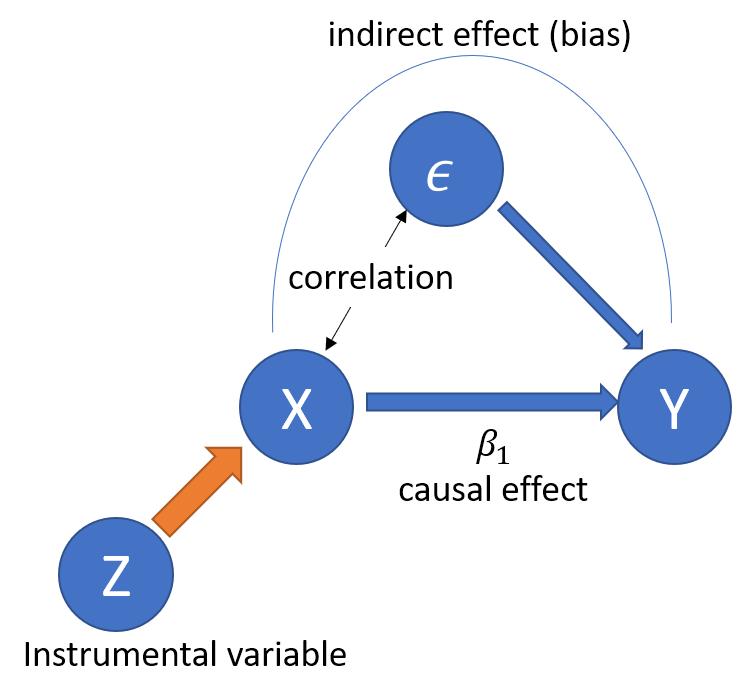
\includegraphics{fig_IV_idea.png}
\caption{Idea IV}
\end{figure}

\end{frame}

\hypertarget{iv-framework}{%
\section{IV framework}\label{iv-framework}}

\begin{frame}{Model}
\protect\hypertarget{model}{}

\begin{itemize}
\tightlist
\item
  We now introduce a general framework with multiple endogenous
  variables and multiple instruments.
\item
  Consider the model \[
  \begin{aligned}
  Y_i = \beta_0 + \beta_1 X_{1i} + \dots + \beta_K X_{Ki} + \beta_{K+1} W_{1i} + \dots + \beta_{K+R} W_{Ri} + u_i, 
  \end{aligned}
  \] with \(i=1,\dots,n\) is the general instrumental variables
  regression model where

  \begin{itemize}
  \tightlist
  \item
    \(Y_i\) is the dependent variable
  \item
    \(\beta_0,\dots,\beta_{K+R}\) are \(1+K+R\) unknown regression
    coefficients
  \item
    \(X_{1i},\dots,X_{Ki}\) are \(K\) endogenous regressors:
    \(Cov(X_{ki}, u_i) \neq 0\) for all \(k\).
  \item
    \(W_{1i},\dots,W_{Ri}\) are \(R\) exogenous regressors which are
    uncorrelated with \(u_i\). \(Cov(W_{ri}, u_i) = 0\) for all \(r\).
  \item
    \(u_i\) is the error term
  \item
    \(Z_{1i},\dots,Z_{Mi}\) are \(M\) instrumental variables
  \end{itemize}
\item
  I will discuss conditions for valid instruments later.
\end{itemize}

\end{frame}

\begin{frame}{Estimation by Two Stage Least Squares (2SLS)}
\protect\hypertarget{estimation-by-two-stage-least-squares-2sls}{}

\begin{itemize}
\tightlist
\item
  We can estimate the above model by \textbf{Two Stage Least Squares
  (2SLS)}
\item
  Step 1: \textbf{First-stage regression(s)}

  \begin{itemize}
  \tightlist
  \item
    Run an OLS regression for each of the endogenous variables
    (\(X_{1i},\dots,X_{ki}\)) on all instrumental variables
    (\(Z_{1i},\dots,Z_{mi}\)), all exogenous variables
    (\(W_{1i},\dots,W_{ri}\)) and an intercept.
  \item
    Compute the fitted values
    (\(\widehat{X}_{1i},\dots,\widehat{X}_{ki}\)).
  \end{itemize}
\item
  Step 2: \textbf{Second-stage regression}

  \begin{itemize}
  \tightlist
  \item
    Regress the dependent variable \(Y_i\) on \textbf{the predicted
    values} of all endogenous regressors
    (\(\widehat{X}_{1i},\dots,\widehat{X}_{ki}\)), all exogenous
    variables (\(W_{1i},\dots,W_{ri}\)) and an intercept using OLS.
  \item
    This gives
    \(\widehat{\beta}_{0}^{TSLS},\dots,\widehat{\beta}_{k+r}^{TSLS}\),
    the 2SLS estimates of the model coefficients.
  \end{itemize}
\end{itemize}

\end{frame}

\begin{frame}{Intuition}
\protect\hypertarget{intuition}{}

\begin{itemize}
\tightlist
\item
  Why does this work? Let's go back to the simple example with 1
  endogenous variable and 1 IV.
\item
  In the first stage, we estimate\\
  \[
  x_i = \pi_0 + \pi_1 z_i + v_i
  \] by OLS and obtain the fitted value
  \(\widehat{x}_i = \widehat{\pi}_0 + \widehat{\pi}_1 z_i\).
\item
  In the second stage, we estimate \[
  y_i = \beta_0 + \beta_1 \widehat{x}_i + u_i
  \]
\item
  Since \(\widehat{x}_i\) depends only on \(z_i\), which is uncorrelated
  with \(u_i\), the second stage can estimate \(\beta_1\) without bias.
\item
  Can you see the importance of both independence and relevance
  asssumption here? (More formal discussion later)
\end{itemize}

\end{frame}

\hypertarget{conditions-for-iv}{%
\section{Conditions for IV}\label{conditions-for-iv}}

\begin{frame}{Conditions for Valid IVs: Necessary condition}
\protect\hypertarget{conditions-for-valid-ivs-necessary-condition}{}

\begin{itemize}
\tightlist
\item
  Depending on the number of IVs, we have three cases

  \begin{enumerate}
  \tightlist
  \item
    Over-identification: \(M > K\)
  \item
    Just identification{]} \(M=K\)
  \item
    Under-identification \(M < K\)
  \end{enumerate}
\item
  The necessary condition is \(M \geq K\).

  \begin{itemize}
  \tightlist
  \item
    We should have more IVs than endogenous variables!!
  \end{itemize}
\end{itemize}

\end{frame}

\begin{frame}{Sufficient condition}
\protect\hypertarget{sufficient-condition}{}

\begin{itemize}
\tightlist
\item
  How about sufficiency?
\item
  In a general framework, the sufficient condition for valid instruments
  is given as follows.

  \begin{enumerate}
  \tightlist
  \item
    \textbf{Independence}: \(Cov( Z_{mi}, \epsilon_i) = 0\) for all
    \(m\).
  \item
    \textbf{Relevance}: In the second stage regression, the variables \[
      \left( \widehat{X}_{1i},\dots,\widehat{X}_{ki}, W_{1i},\dots,W_{ri}, 1 \right)
      \] are not perfectly multicollinear.
  \end{enumerate}
\item
  What does the relevance condition mean?
\end{itemize}

\end{frame}

\begin{frame}{Relevance condition}
\protect\hypertarget{relevance-condition}{}

\begin{itemize}
\tightlist
\item
  In the simple example above, The first stage is\\
  \[
  x_i = \pi_0 + \pi_1 z_i + v_i
  \] and the second stage is \[
  y_i = \beta_0 + \beta_1 \widehat{x}_i + u_i
  \]
\item
  The second stage would have perfect multicollinarity if \(\pi_1 = 0\)
  (i.e., \(\widehat{x}_i = \pi_0\)).
\item
  Back to the general case, the first stage for \(X_k\) can be written
  as \[
  X_{ki} = \pi_0 + \pi_1 Z_{1i} + \cdots + \pi_M Z_{Mi} + \pi_{M+1} W_{1i} + \cdots + \pi_{M+R} W_{Ri}
  \] and one of \(\pi_1 , \cdots, \pi_M\) should be non-zero.
\item
  Intuitively speaking, \textbf{the instruments should be correlated
  with endogenous variables after controlling for exogenous variables}
\end{itemize}

\end{frame}

\begin{frame}{Check Instrument Validity: Relevance}
\protect\hypertarget{check-instrument-validity-relevance}{}

\begin{itemize}
\tightlist
\item
  Instruments are \textbf{weak} if those instruments explain little
  variation in the endogenous variables.
\item
  Weak instruments lead to

  \begin{enumerate}
  \tightlist
  \item
    imprecise estimates (higher standard errors)
  \item
    The asymptotic distribution would deviate from a normal distribution
    even if we have a large sample.
  \end{enumerate}
\item
  Here is a rule of thumb to check the relevance conditions.
\end{itemize}

\end{frame}

\begin{frame}

\begin{itemize}
\tightlist
\item
  Consider the case with one endogenous variable \(X_{1i}\).
\item
  The first stage regression\\
  \[
  X_k = \pi_0 + \pi_1 Z_{1i} + \cdots + \pi_M Z_{Mi} + \pi_{M+1} W_{1i} + \cdots + \pi_{M+R} W_{Ri}
  \]
\item
  And test the null hypothesis \[
  \begin{aligned}
  H_0 & : \pi_1 = \cdots = \pi_M = 0 \\ 
  H_1 & : otherwise
  \end{aligned}
  \]

  \begin{itemize}
  \tightlist
  \item
    This is F test (test of joint hypothesis)
  \end{itemize}
\item
  If we can reject this, we can say no concern for weak instruments.
\item
  A rule of thumbs is that the F statistic should be larger than 10.
\end{itemize}

\end{frame}

\begin{frame}{Independence (Instrument exogeneity)}
\protect\hypertarget{independence-instrument-exogeneity}{}

\begin{itemize}
\tightlist
\item
  Arguing for independence is hard and a key in empirical analysis.
\item
  Justification of this assumption depends on a context, institutional
  features, etc\ldots{}
\item
  We will see this through examples in the next chapter.
\end{itemize}

\end{frame}

\end{document}
